
\chapter{Architektura a technologie} \label{archtech}

\LaTeX
\section{Architektura řešení} \label{architektura_reseni}

\begin{figure} \centering
  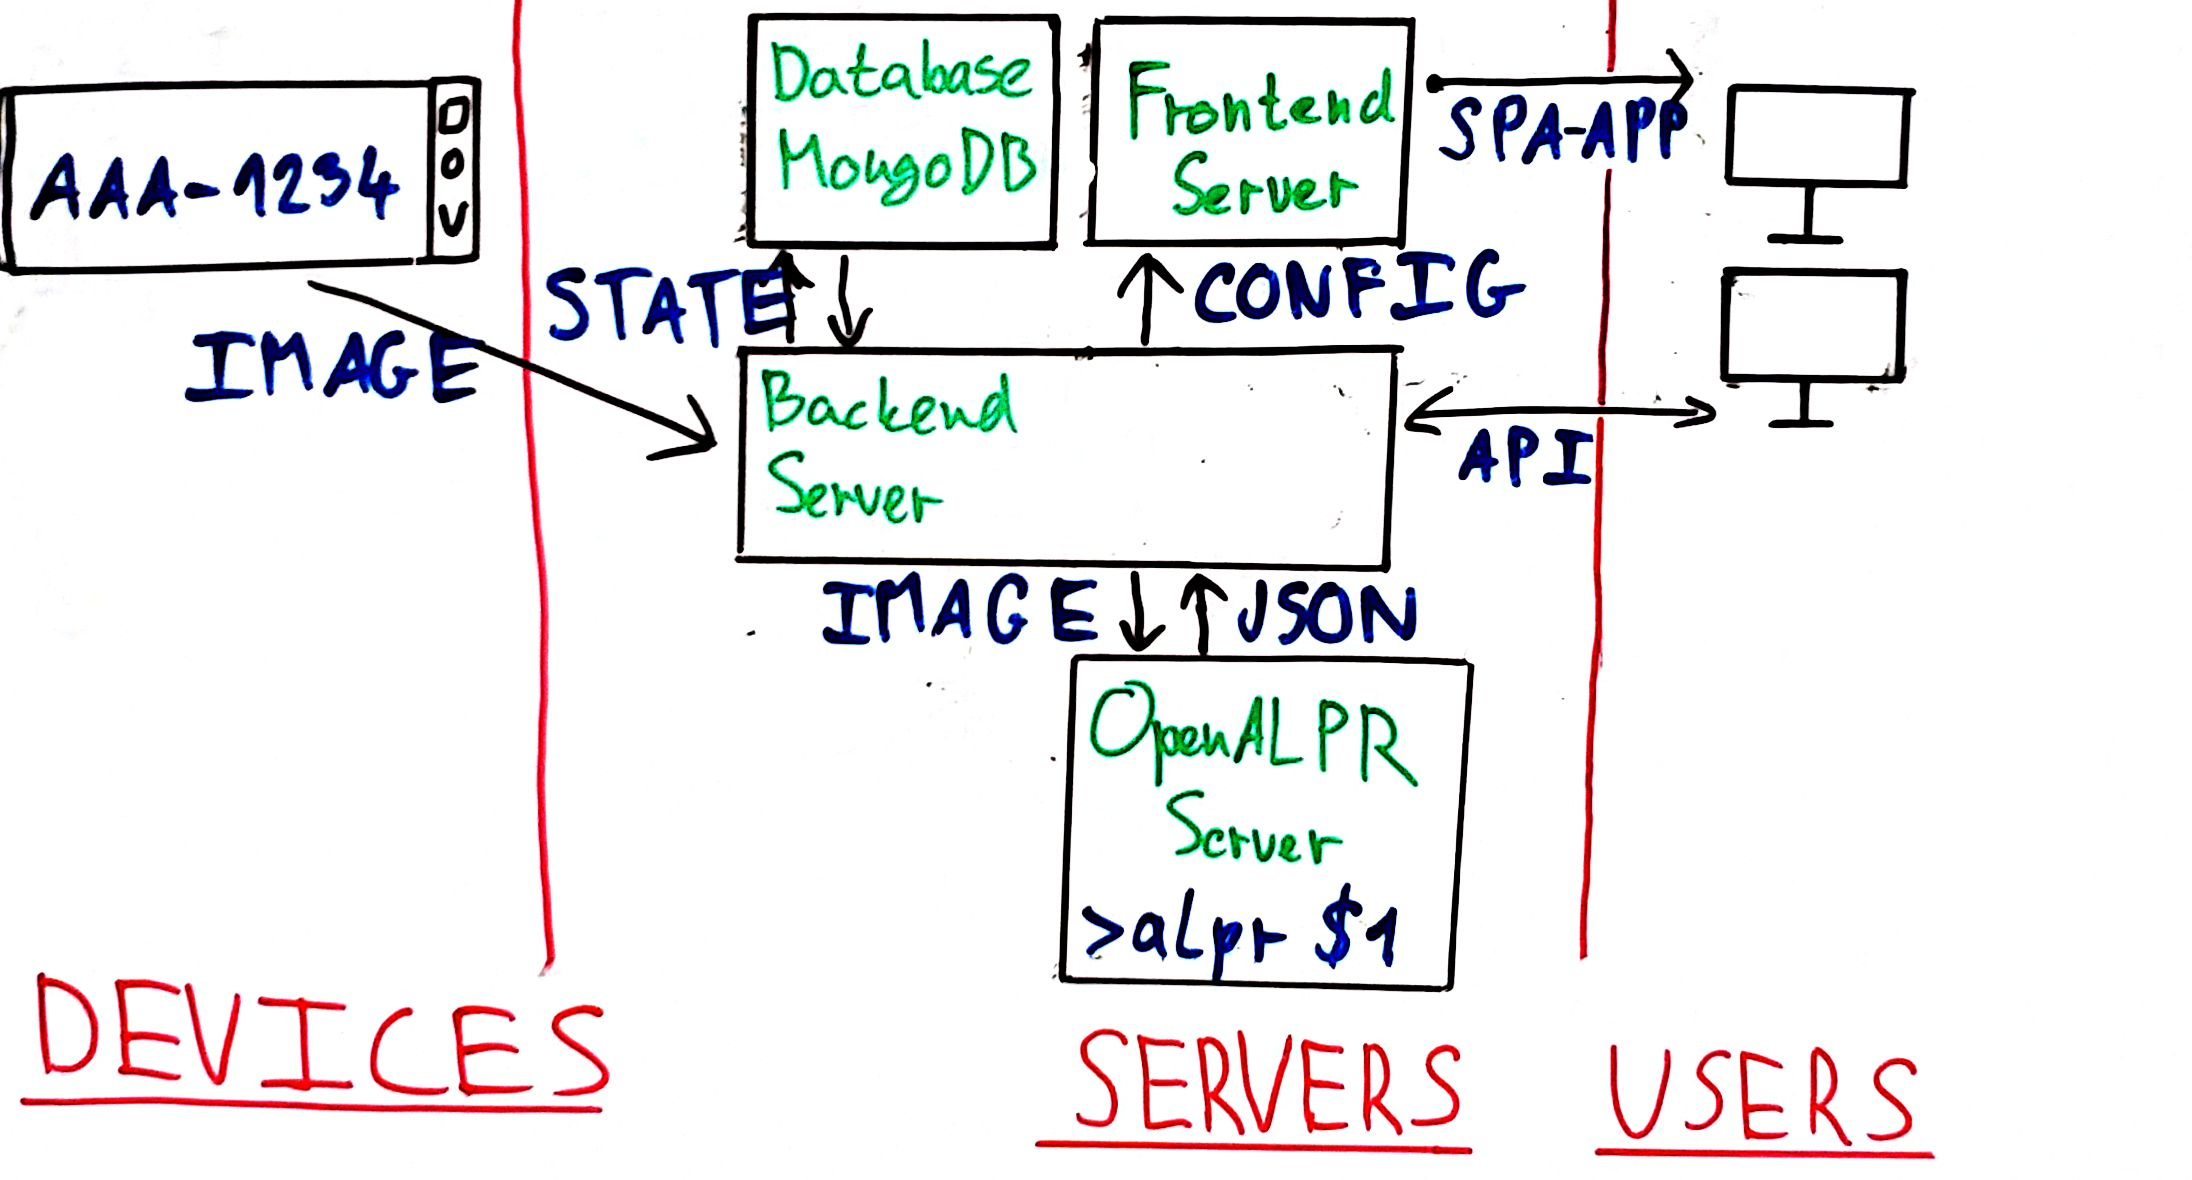
\includegraphics[width=145mm]{../img/architecture_drawing.jpg}
  \caption{Diagram komponent a jejich komunikace.}
  \label{fig:architecture_drawing}
\end{figure}

Parkovací systém se zkládá z následujících částí, které si nyní popíšeme stručně a detailněji později.
Části spolu komunikují pomocí HTTP.
Obrázek \ref{fig:architecture_drawing} ukazuje tyto části a nastiňuje způsob komunikace.

\begin{itemize}
  \item \textbf{Backend} je středobodem celé aplikace -- komunikuje se všemy ostatními komponentami.
        Zajišťuje business logiku aplikace, autentizaci i autorizaci uživatelů a perzistenci dat do \textbf{Databáze}.
  \begin{itemize}
    \item \textbf{Databáze} slouží k ukládání a čtení dat.
    \item \textbf{OpenALPR Server} (převzato z https://github.com/gerhardsletten/express-openalpr-server) je server, jenž obstarává přístup
          ke knihovně OpenALPR (https://github.com/openalpr/openalpr), která rozpoznává SPZ, přes protokol http.
  \end{itemize}
  \item \textbf{Mobilní aplikace} posílá obrazová data na \textbf{Backend}, kde jsou zpracována. Je určena pro platformu Android.
  \item \textbf{Frontend} je rozhraní mezi celým systémem a správcem parkoviště a dalšího personálu.
\end{itemize}

\section{Technologie}

\subsection{Databáze}

Databáze MongoDB, která byla vybrána, protože data se budou převážně zapisovat a bude potřeba v nich rychle hledat a provádět agregační dotazy.
Mimo jiné umožňuje provoz několika spolupracujících instancí, zálohování apod \citep[viz][]{MongoDB}.

\subsection{Backend} \label{backend}

Jako programovací jazyk pro \textbf{Backend} byl zvolen staticky typovaný Typescript kvůli rychlosti vývoje
a množství knihoven, které poskytuje ekosystém Node.js.

Pro definici databázových modelů a komunikaci s MongoDB byla kvůli své vyspělosti a skvělé funkcionalitě zvolena
knihovna mongoose.

Primárním způsobem komunikace s \textbf{Frontend}
je dotazovací jazyk GraphQL, který přináší ucelený popis poskytovaných dat pomocí kontroly typů,
expresivních dotazů, jejichž odpověď má stejný "tvar" v JSON formátu.
Obrázek \ref{fig:graphql_example} ukazuje dotaz hledání uživatele podle jména.

\begin{figure} \centering
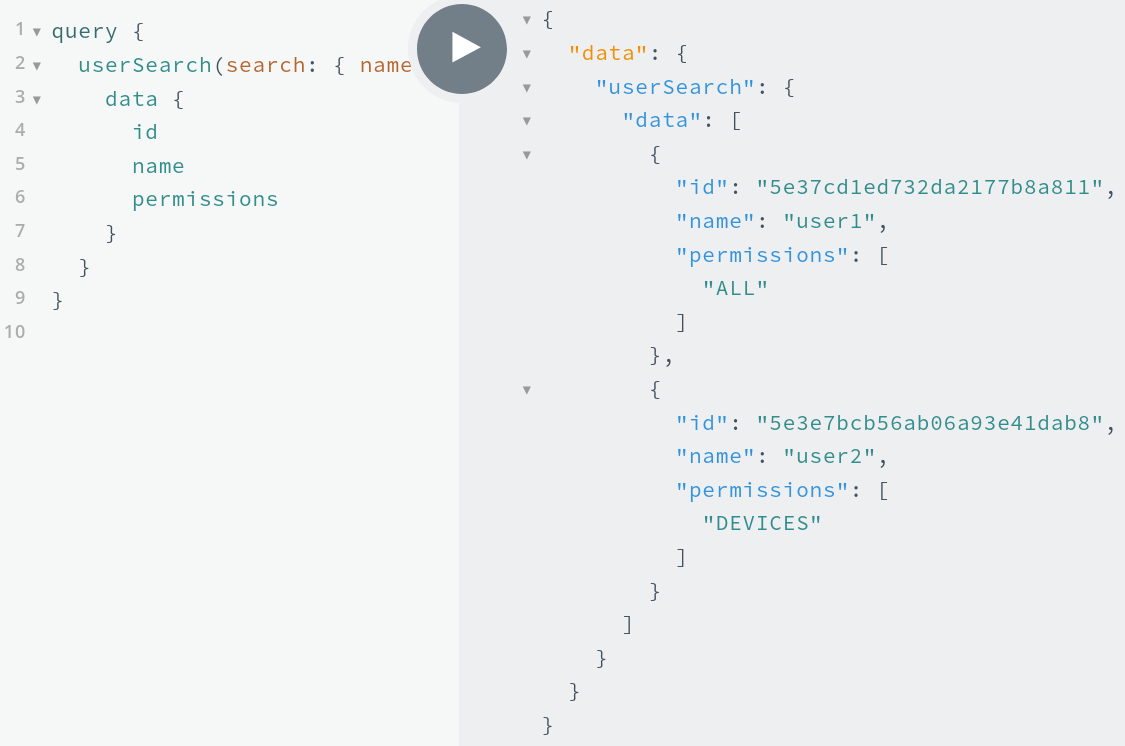
\includegraphics[width=145mm]{../img/graphql_example.png}
\caption{Příklad GraphQL dotazu (vlevo) a odpovědi (vpravo). Screenshot z nástroje GraphQL Playground.}
\label{fig:graphql_example}
\end{figure}

Model uživatele může mít i další atributy, ale GraphQL vrátí přesně ty údaje, na které se uživatel zeptal.
Tento triviální příklad neukazuje další funkce jako mutace dat, dědičnost typů, více dotazů v jednom http dotazu
a mnoho dalších.
GraphQL je pouze specifikace vytvořená společností Facebook a má několik
implementací. Pro tento projekt byla zvolena implementace Apollo \citep[viz][]{Apollo}. Detailní informace jsou dostupné na oficiálních
stránkach https://graphql.org/.

Jelikož GraphQL posílá odpovědi v JSON, není vhodné na posílání obrázků. Je to možné za využití base64 kódování,
ale přes síť se přenese více bytů, než při použití obvyklého způsobu přes HTTP. Z toho důvodu pro posílání
obrázků (např. QR kódu pro Frontend pro autentifikaci zařízení nebo zaznamenané znímky SPZ) bude mít Backend i
klasické REST endpointy.

\subsection{Frontend} \label{frontend}

Pro \textbf{Frontend} byl jako u \textbf{Backend} vybrán Typescript ze stejných důvodů. Webové rozhraní
je takzvaná SPA (z angl. Single-Page-Application), což znamená, že uživateli se obsah mění dynamicky
bez načítání dalších stránek.
Renderování zajišťuje knihovna React, která od klasického přístupu, kdy se odděluje HTML a Javascript do separátních
souborů, mandatuje, že v jednom souboru je jedna komponenta se vším svým HTML a logikou ve formě Javascriptu nebo
Typescriptu. Pomocí další knihovny typestyle pak můžeme do stejného souboru psát i typované CSS.
Aby bylo možné snadno sdílet mezi komponentami stav, byla pro takzvaný state-management zvolena knihovna Redux.
Diagram na obrázku \ref{fig:react_redux_dataflow} ukazuje tok dat mezi Reactem a Reduxem.

Jelikož je aplikace vyvíjena pro správce systému a ne pro velké množství uživatelů, můžeme si dovolit
klást menší nároky na velikost aplikace (tj. můžeme přidávat i velké knihovny), což velice usnadní vývoj za
nízkou cenu.

\begin{figure}[!htb] \centering
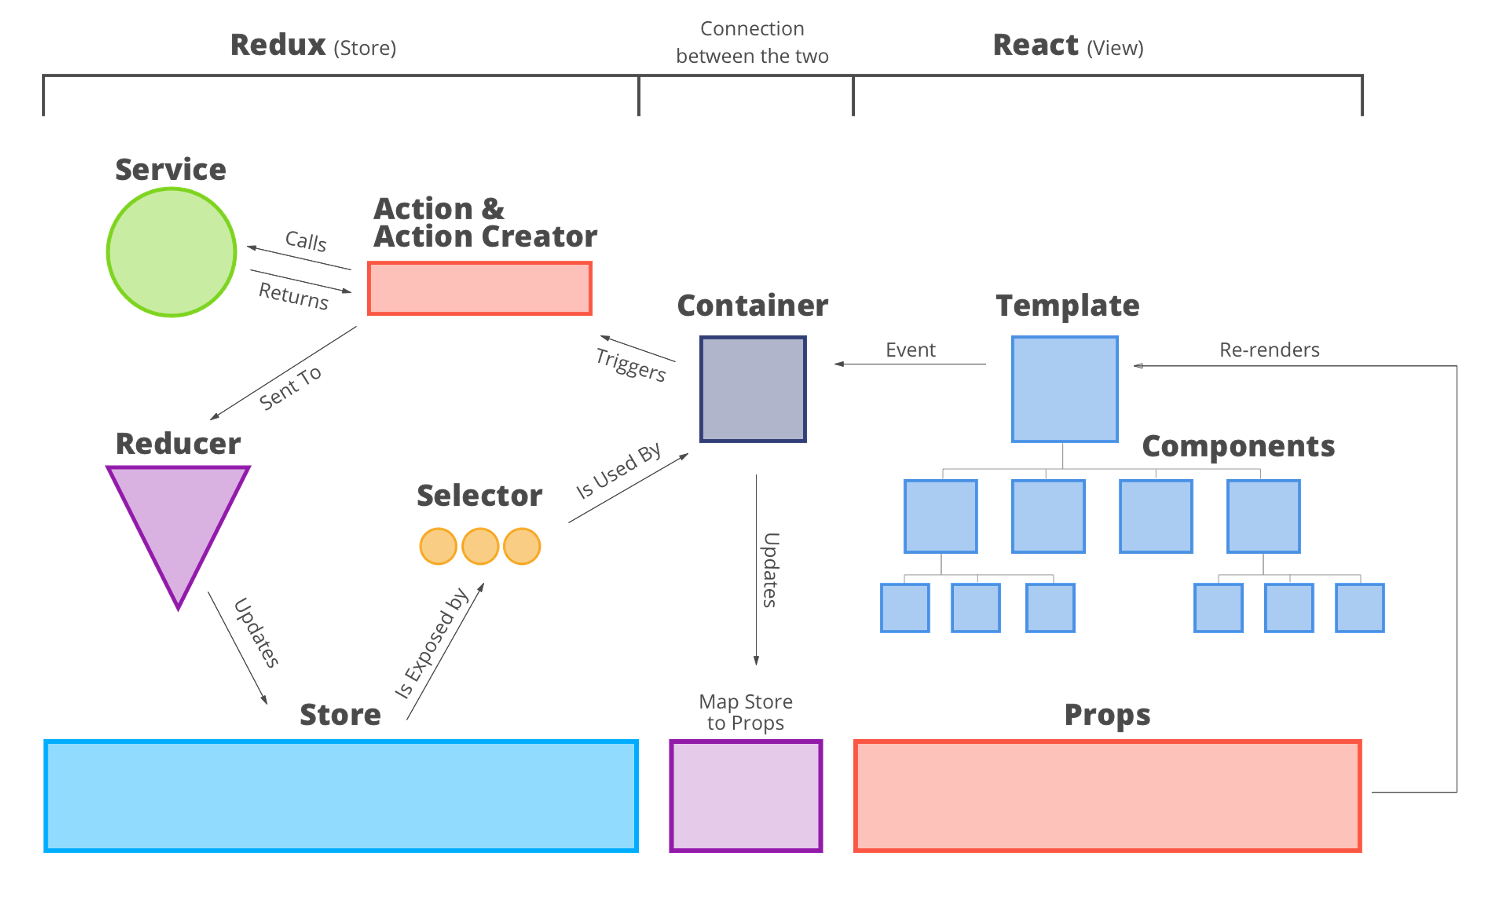
\includegraphics[width=145mm]{../img/react-redux-architecture.png}
\caption{Spojení React a Redux. \citep[viz][]{react_redux_dataflow}}
\label{fig:react_redux_dataflow}
\end{figure}

\subsection{Mobilní aplikce} \label{mobile_app}

\textbf{Mobilní aplikace}, která je určena pro platformu Android, měla volbu jazyka omezenou na Javu, Kotlin a C++.
Rychlost C++ není potřeba a navíc autor s tímto nízkoúrovňovým jazykem nemá takové zkušenosti.
Kotlin oproti Javě umožňuje přímočarejší přístup k prkům uživatelského rozhraní, a proto byl zvolen.

Jediným úkolem \textbf{Mobilní aplikace} je v pravidelném intervalu pořídit snímek fotoaparátem a poslat ho na
\textbf{Backend}, který jej patřičně zpracuje.

\subsection{Detekce SPZ}

Detekci SPZ bude zajišťovat knihovna OpenALPR \citep[viz][]{OpenALPR}, jejímž vstupem je obrázek a popřípadě
parametry jako úhel kamery apod. Ke zbytku aplikace bude připojena malým HTTP serverem, jenž byl převzán a upraven
\citep[viz][]{OpenALPR_Server}.
Ten umožňuje poslat pomocí protokolu HTTP obrázek a obdržet JSON s SPZ daty a souřadnicemi detekované SPZ.
Samotný server ke knihovně přistupuje zavoláním binárky \textit{alpr}, který jako argument přijme cestu k
obrázku, ve kterém hledáme SPZ. Alternativní a lepší způsob přístupu by bylo mít v Node.js přímo takzv.
\textit{language-binding}, ale to se autorovi (a mnoho dalším, kteří se o to pokoušeli) nepodařilo.

\section{Metodika vývoje}

Nejprve se vyvine veškerá funkcionalita v základní podobě
(na způsob MVP -- z angl. Minimal-Viable-Product) a později se vše vyhladí a zlepší. To však neznamená,
že bychom si nedali záležet na kvalitním a udržitelném kódu, naopak. Cílem je mít flexibilní základ,
na kterém lze stavět. Pro klidný spánek budeme psát dle uvážení automatizované testy, abychom předešli
nežádoucímu chování aplikace (takzvaná regrese) po úpravě kódu.

Backend i frontend budou vyvinuty současně. Dokud není mobilní aplikace pro zařízení, lze ji simulovat
například nástrojem curl.
